\section{Robustness and Practical Implications}\label{sec:discussion}\label{sec:robustness}
\subsection{Robustness}
\label{sec:results-robustness}

Of the seven preregistered robustness families (\S\ref{sec:robustness}), six were computed (five in the ranking-correlation, temporal-robustness, and sample-complexity outputs below, and a sixth, \texttt{LEAVE\_ONE\_POLICY\_FAMILY\_OUT}, in the telemetry-explanation analysis of \S\ref{sec:telemetry-explanation}). The seventh, \texttt{METRIC\_DEFINITION\_SENSITIVITY}, was never implemented; we disclose this as a protocol gap rather than perform a post hoc analysis after the results were already known.

\begin{itemize}
  \item \textbf{\texttt{PRIMARY\_ONLY}.} Identical to the headline result
    by construction: the ranking correlations artifact already restricts
    every comparison to the 11-policy PRIMARY panel
    (\S\ref{sec:cross-source-rankings}), never mixing in the two
    \texttt{STYLE\_APPROXIMATION} robustness policies.
  \item \textbf{\texttt{LEAVE\_ONE\_SOURCE\_OUT}.} Excluding BurstGPT
    leaves only the Azure-2024/Bailian-Qwen pair, whose mean tau-b is
    $0.948$ -- close to the ceiling. Excluding Azure-2024 or Bailian/Qwen
    each leaves a BurstGPT-involving pair, with mean tau-b $0.618$ and
    $0.633$ respectively. This is the same asymmetry as
    \S\ref{sec:cross-source-rankings}, now stated per excluded source: the
    headline portability figure is high specifically because two of the
    three sources agree strongly, and is pulled down specifically by
    BurstGPT, not uniformly by all three sources.
  \item \textbf{\texttt{LOAD\_CALIBRATION\_SENSITIVITY}.} Reported in
    \S\ref{sec:load-conditioning}: mean tau-b changes by less than $0.01$
    between the four- and six-region grids.
  \item \textbf{\texttt{TEMPORAL\_SPLIT\_SENSITIVITY}.} The BurstGPT
    bisect-vs-tercile comparison from \S\ref{sec:temporal}; both split
    definitions are reported side by side in the preserved table rather
    than collapsed into one number.
  \item \textbf{\texttt{WINDOW\_SIZE\_SENSITIVITY}.} Despite its name,
    this item is the window-\emph{count} subsampling ladder of
    \S\ref{sec:sample-complexity}, not a requests-per-window sweep
    (\S\ref{sec:window-size}), and is not separately recomputed here.
  \item \textbf{\texttt{LEAVE\_ONE\_POLICY\_FAMILY\_OUT}.} Excluding any
    single one of the ten frozen mechanism families changes the headline
    mean tau-b only modestly, from $0.707$ (excluding the classical
    arrival-order family) to $0.792$ (excluding the SLO-aware family),
    against the full-panel baseline of $0.733$. No single mechanism
    family's removal collapses or inflates the headline portability
    figure -- the source-pair-driven pattern of
    \S\ref{sec:cross-source-rankings} is not an artifact of any one
    policy family dominating the panel.
\end{itemize}

\subsection{Finite-Corpus Ranking Recovery}
\label{sec:sample-complexity}

\paragraph{Scope}
\label{sec:sample-complexity-motivation}

The reference is the frozen 40-window ranking, not an unknown population optimum. Recovery is conditional on this finite corpus and the historical tie rule.

\paragraph{Design and results}
\label{sec:sample-complexity-design}

The $0.9$ recovery probability used throughout this section is a
pre-registered benchmark reporting target, fixed before any
sample-complexity output was computed: it provides one interpretable,
high-recovery criterion for comparing sources and metrics against each
other, and is not asserted to be a universal statistical-significance
level or a field-standard adequacy cutoff for scheduler benchmarking.

For the PRIMARY metric, recovery of the exact $n=40$ reference ranking is
slow and strongly source-dependent (Figure~\ref{fig:sample-complexity}): BurstGPT never reaches the preregistered
$0.9$ exact-order recovery threshold below the full window budget ($0.2\%$
at $n=5$, rising only to $56.6\%$ at $n=30$), Bailian/Qwen similarly does
not cross $0.9$ before the $n=40$ ceiling ($64.0\%$ at $n=30$), while Azure-2024
crosses the threshold already at $n=30$ ($98.8\%$). None of the three
sources reaches $0.9$ exact-order recovery at $n \in \{5,10,20\}$. Because
$n=40$ is the size of the full reference pool itself, exact recovery at
$n=40$ is $1.0$ by construction (sampling all 40 windows without
replacement reproduces the reference exactly) and is not an informative
data point on its own; the informative content is in how slowly each
source's curve rises toward that trivial ceiling.

Top-1 recovery (does the resampled subset identify the single
best-performing PRIMARY-panel policy correctly) is a materially easier
question than exact-order recovery for two of the three sources: Azure-2024
and Bailian/Qwen both exceed $0.9$ top-1 recovery already at $n=5$
($96.6\%$ and essentially $100\%$ respectively), even though their
\emph{exact}-order recovery at $n=5$ is only $35.0\%$ and $14.6\%$. For
these two sources, identifying the single best policy requires far less
evidence than reconstructing the complete 11-policy ordering. BurstGPT
shows no such gap: its top-1 recovery is comparably slow to its
exact-order recovery ($13.0\%$ at $n=5$, $74.2\%$ at $n=30$), remaining below
$0.9$ until the trivial $n=40$ ceiling -- consistent with
\S\ref{sec:cross-source-rankings}'s finding that BurstGPT is the source
whose relative ordering is hardest to pin down. Comparing a concentrated
(single-source-heavy) against a distributed (evenly-spread-across-sources)
window budget of equal total size, the distributed budget achieves higher
mean Kendall's tau-b against the reference ranking ($0.986$) than the
concentrated budget ($0.940$) for the primary metric -- spreading a fixed
evaluation budget across sources recovers the reference ranking more
reliably than concentrating it in one source.

\begin{figure}[h]
\centering
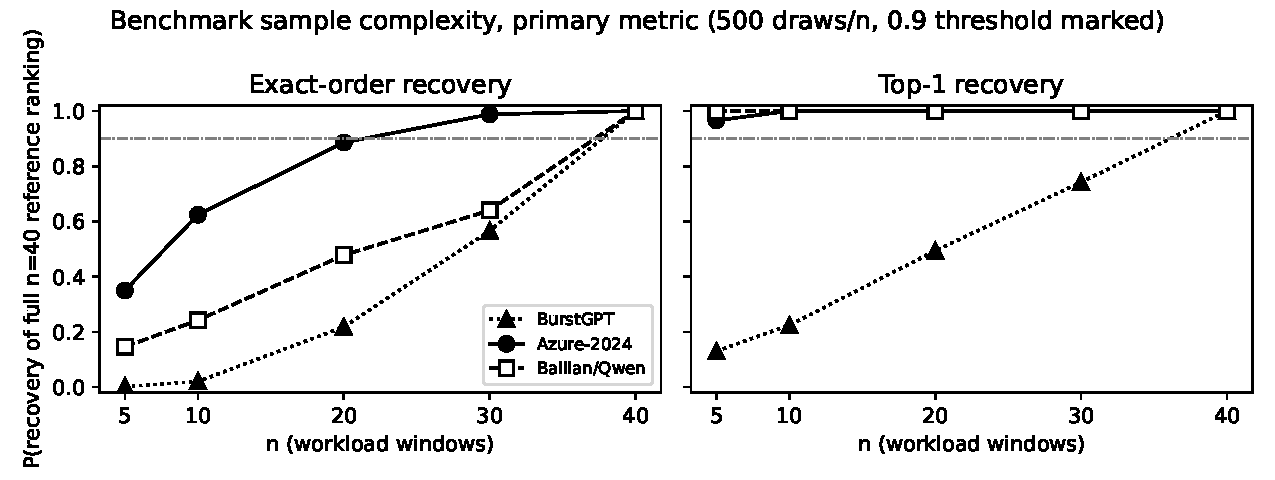
\includegraphics[width=\textwidth]{figures/fig3_sample_complexity_curves.pdf}
\caption{Benchmark sample-complexity recovery curves, PRIMARY metric, 500
draws per $n$, sampling without replacement. Left: exact-order recovery of
the full $n=40$ reference ranking. Right: top-1 recovery. The $0.9$
threshold is marked. Computed from the frozen sample complexity artifact.}
\label{fig:sample-complexity}
\Description{Exact-order and top-choice recovery probabilities at 5, 10, 20, 30 and 40 windows. The full 40-window reference is recovered by construction.}
\end{figure}

This analysis directly answers RQ5 (\S\ref{sec:rq}) and depends on the full
primary outcome matrix (\S\ref{sec:results}); it is not run on the earlier,
smaller discriminability pilot (\S\ref{sec:stage0}).
\subsection{SLO-Definition Sensitivity}
\label{sec:results-slo}

As disclosed in \S\ref{sec:slo-sensitivity-gap}, this check was never part
of the preregistered protocol; we report it here as the post-campaign
extension it was actually run as: three alternative SLO-synthesis
multipliers (\texttt{tight\_10x}, \texttt{primary\_20x} -- this study's own
convention -- and \texttt{loose\_40x}) applied across the 5 load regions
that contain at least one PRIMARY-metric supported reversal (excluding
\texttt{LOW}, which accounts for 0 of the 36 supported reversals and so
has nothing for a sensitivity check to stress-test), evaluating $11$
policies $\times$ $120$ total windows $\times$ $5$ regions $\times$ $3$
variants ($19{,}800$ input rows according to the preserved extension status), with every seed held identical to
\S\ref{sec:results}.

\textbf{Ranking robustness.} Across the $30$ (source, region, variant)
conditions compared against the study's primary SLO convention, rank
correlation stays high under either alternative (median Kendall's
$\tau_b = 0.872$, range $[0.533, 1.000]$); the single top-ranked policy
nonetheless changes under an alternative SLO definition in $13/30$ ($43\%$)
of conditions.

\textbf{Reversal persistence.} We check the 36 PRIMARY-metric supported reversals from \S\ref{sec:reversals} against the alternative definitions. Because there are 3 SLO variants (tight, primary, loose), there are $36 \times 3 = 108$ mathematical comparisons in the artifact's persistence matrix, of which $36$ are identity checks against the primary definition itself (all 36 trivially persist). Restricting focus to the $72$ scientifically meaningful non-trivial comparisons against the alternative definitions: $52/72$ ($72\%$) persist, $6/72$ ($8\%$) change direction, $10/72$ ($14\%$) remain the same direction but fall below the practical-margin threshold under the alternative definition, and $4/72$ ($6\%$) become statistically indistinguishable from zero. The six direction changes contradict a claim of invariant reversal direction under alternative deadlines. A non-trivial minority ($20/72$, $28\%$) are sensitive to the SLO-definition
choice -- disclosed here as a caveat on those specific reversals, not
grounds to discard them.


\subsection{Explanations and unresolved questions}\label{sec:telemetry-explanation}\label{sec:results-rq3-pilot}\label{sec:slo-sensitivity-gap}
The saved descriptor regression has 42 usable fits among 990 records;
no standard errors establish a directional explanatory claim. Source
identity, prompt structure and simulator execution semantics remain
confounded. The descriptive association is not a causal mechanism result
or a deployment selector. The synthetic-to-real pilot is engineering
context only; it does not answer RQ3 at the level of the primary corpus.

The SLO extension was specified after the primary outcomes were known.
The alternative-metric-definition robustness item remains distinct from
that deadline-synthesis extension. Neither replaces a missing prospective
analysis, and requests-per-window sensitivity is still unmeasured.

Practically, a ranking should travel with its implementation identity,
workload/window definition, calibration, metric denominator, tie rule and
uncertainty procedure. Agreement on that record is evidence for the
specific comparison. A changed objective or execution model warrants
reassessment; it does not license assuming a reversal. No held-out
portability predictor or cost-effective recalibration rule is validated here.
